\newpage

\section{Entwürfe, Mockups und Designvorstellungen}

\subsection{Die Level}

\begin{flushright}

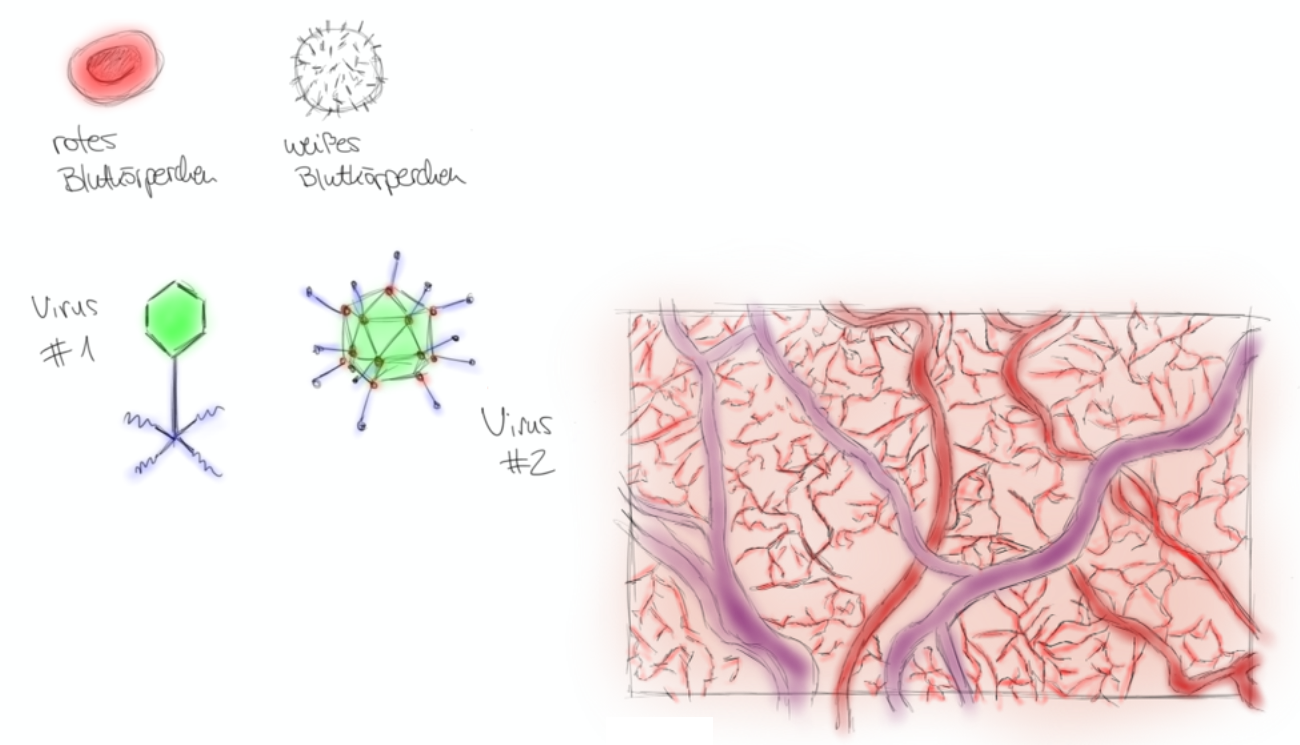
\includegraphics[width=0.88\textwidth]{img/blutlaufbahn.png}\\
\textit{Level 1 - die Rennstrecke in der Blutbahn}\\[3em]

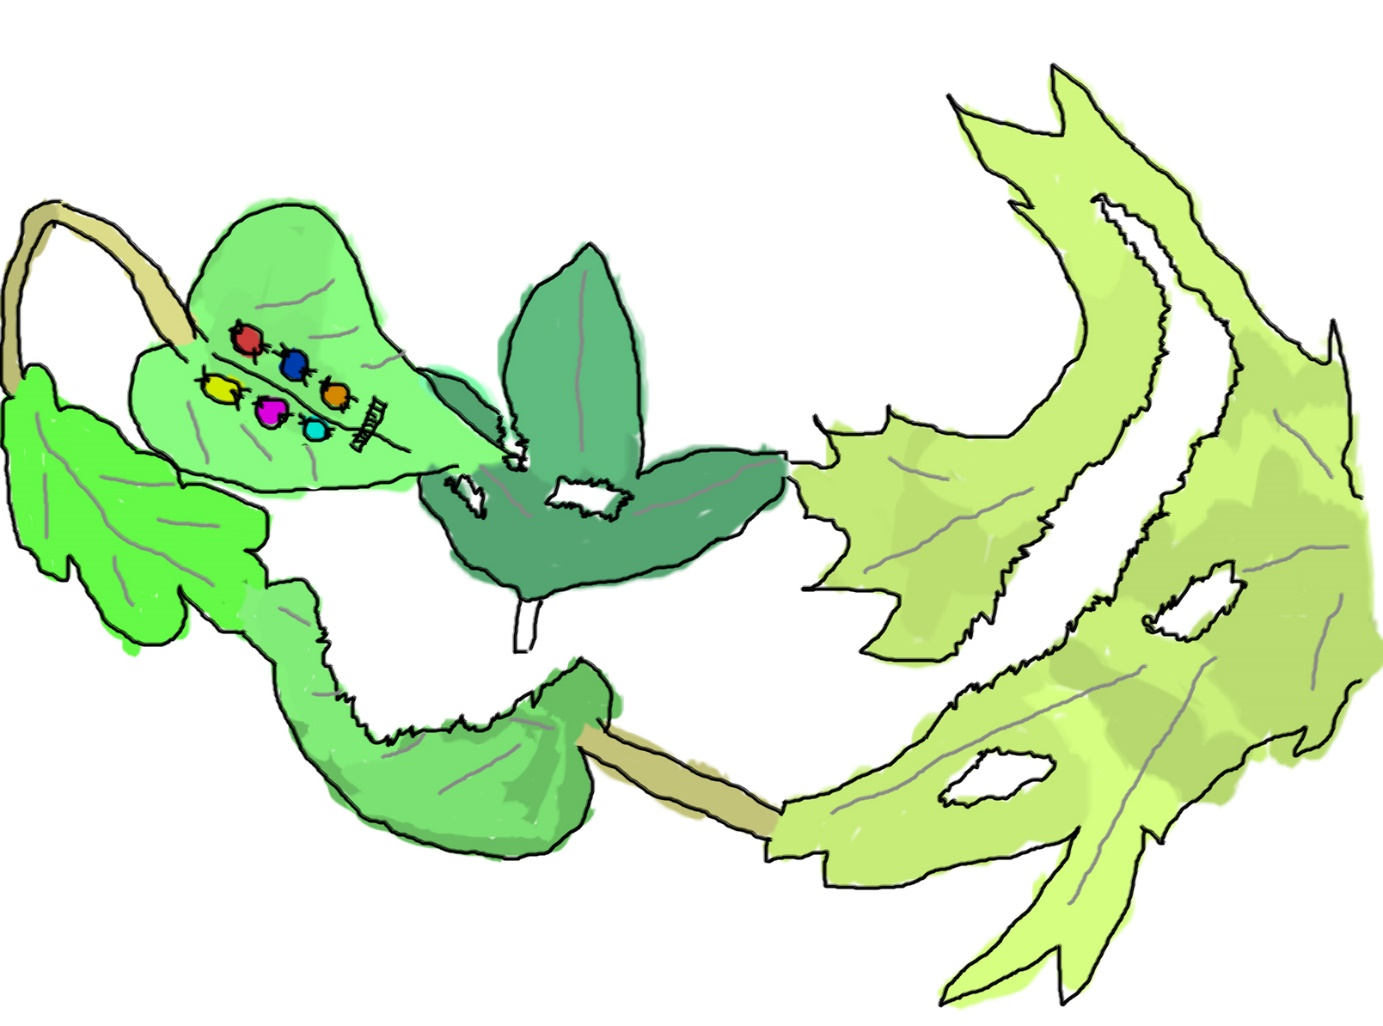
\includegraphics[width=0.88\textwidth]{img/kaefer.png}\\
\textit{Level 2 - eine Blätterstrecke für die Käfer}

\newpage

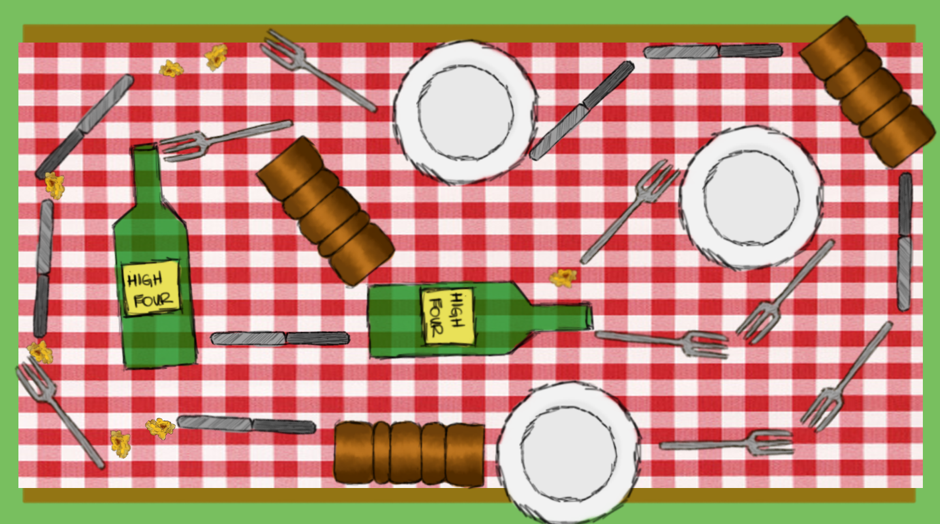
\includegraphics[width=1\textwidth]{img/picknick.png}
\textit{Level 3 - Picknickdecke}\\[3em]

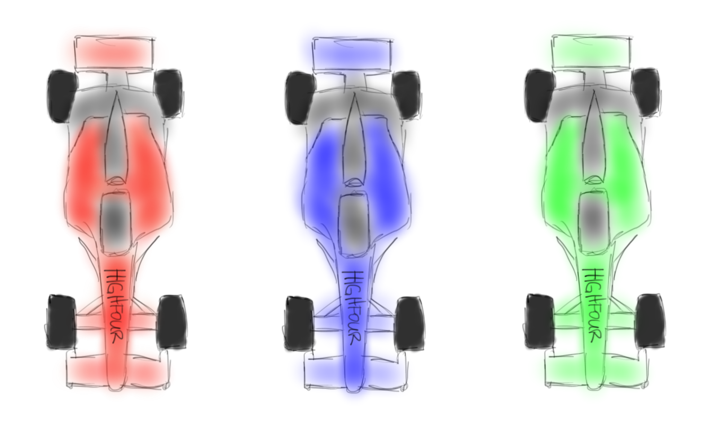
\includegraphics[width=1\textwidth]{img/autos.png}
\textit{Level 3 - ferngesteuerte Autos für das Picknicklevel}

\newpage

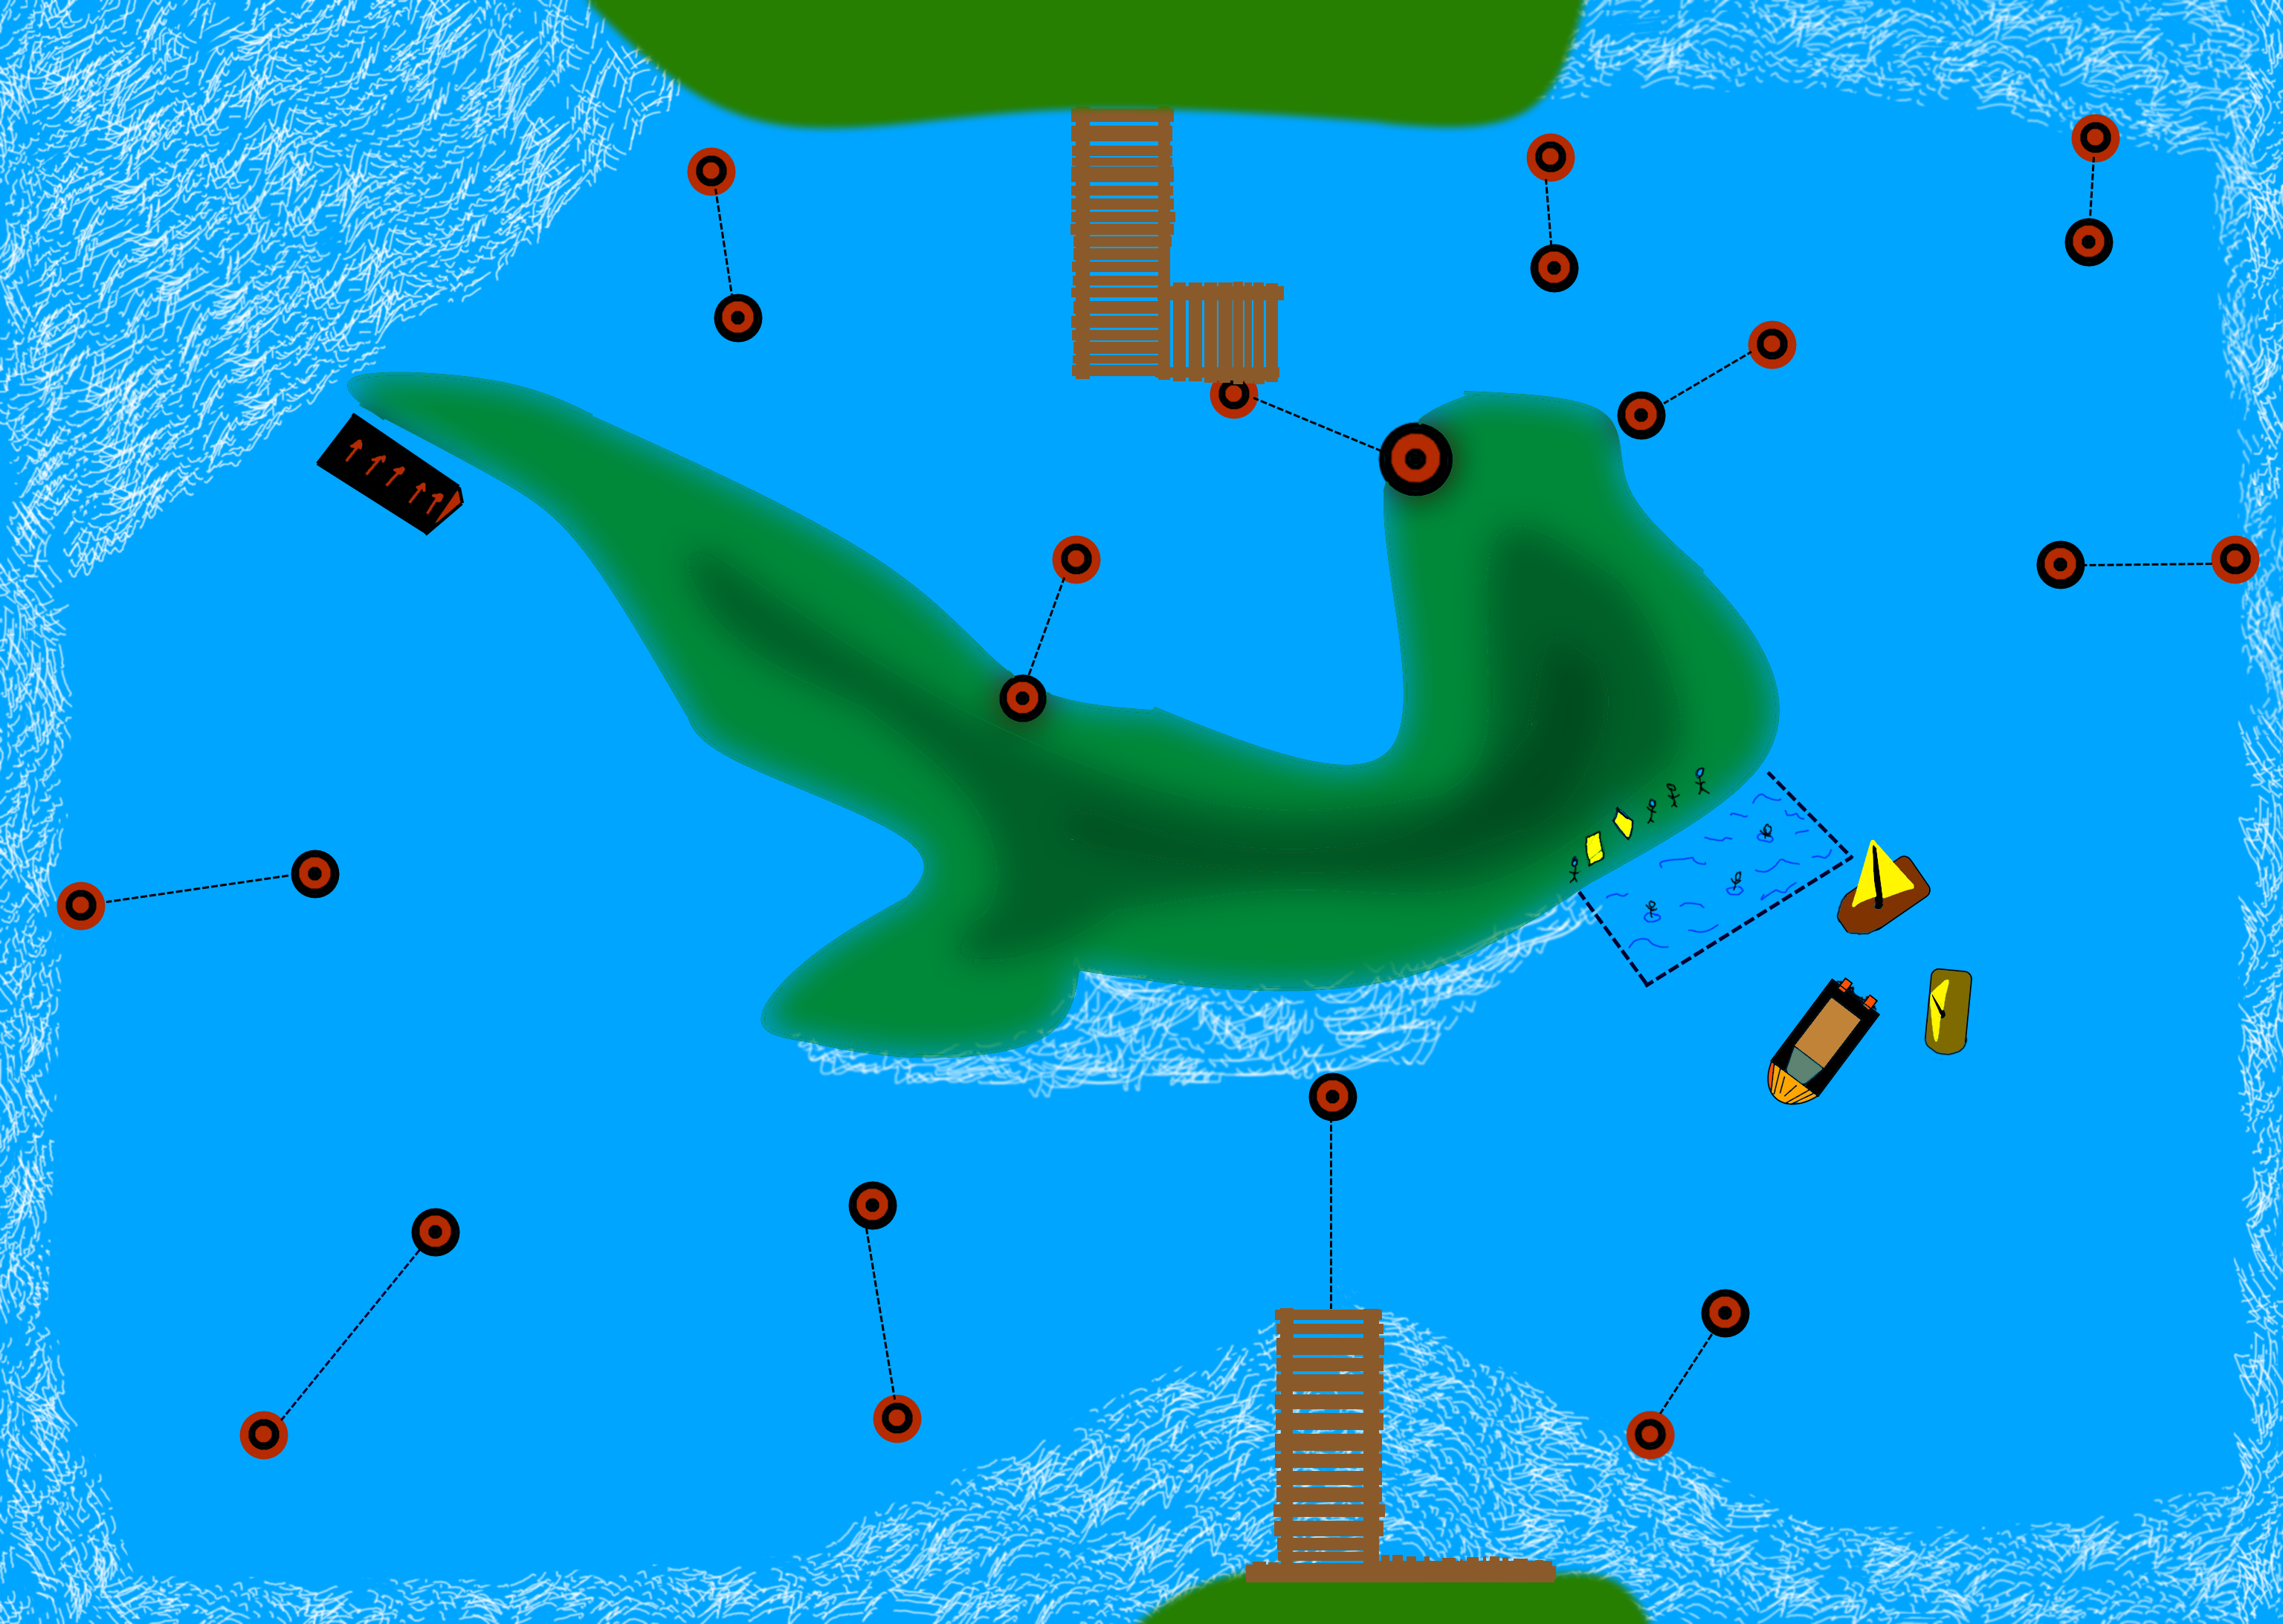
\includegraphics[width=0.95\textwidth]{img/wasserkurs.png}\\
\textit{Level 4 - ein Wasserkurs für die Jetskis}\\[3em]

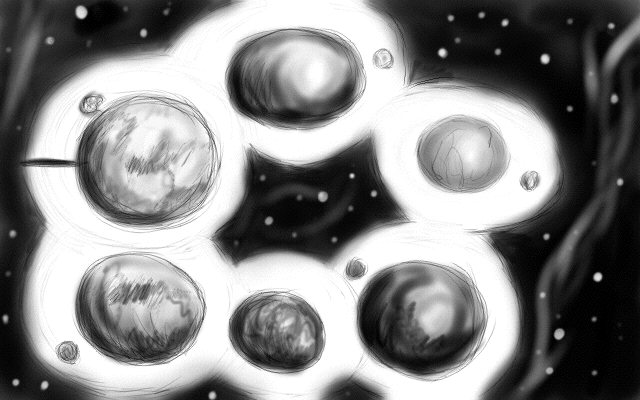
\includegraphics[width=0.95\textwidth]{img/asteroiden.png}\\
\textit{Level 5 - die größte Rennstrecke im All für Asteroiden}

\newpage

\end{flushright}

\subsection{Design}

Als Kontrast zu der Schrift haben wir für die Menüs einen dunklen Hintergrund gewählt, wodurch das wichtige gut lesbar hervorsticht.\\
Als wiederkehrenden gestalterischen Rahmen, der die einzelnen Level und Menüs unseres Spiels zusammenhält, haben wir uns für einen hellblauen Ring mit gleichfarbiger Schrift entschieden.\\
Dieser Ring, ob als „Start“-Knopf oder als Anzeige der Spieleranzahl, stellt zumeist eine Schaltfläche dar. Ausnahme sind u.a. die Kreise, welche verschiedenfarbig ein Foto eines Spielers enthalten. Jene sind vor allem bei jedem Level am oberen Bildschirmrand, je nach aktueller Platzierung, angeordnet, sodass jeder Spieler jeder Zeit einsehen kann, an welcher Position sich er selbst und seine Mitspieler befinden.\\
Unter anderem wird der Fotoring auch dafür verwendet, den Gewinner zum Schluss eines Rennens anzuzeigen.\\
Die Farbe eines Spielers ist vorentschieden, an die Spieleranzahl gebunden und entscheidet sich für jeden Spieler beim Verbinden des mobilen Gerätes mit dem Desktop-PC, je nach Reihenfolge des Verbindungsaufbaus der Spieler.

\begin{flushright}

\subsection{Die Menübildschirme}

\ \\

\includegraphics[width=0.9\textwidth]{img/connect.png}\\
\textit{Die Verbindung der Mobilgeräte}

\newpage


\includegraphics[width=0.9\textwidth]{img/hauptmenu.png}\\
\textit{Das Hauptmenü}\\[2em]

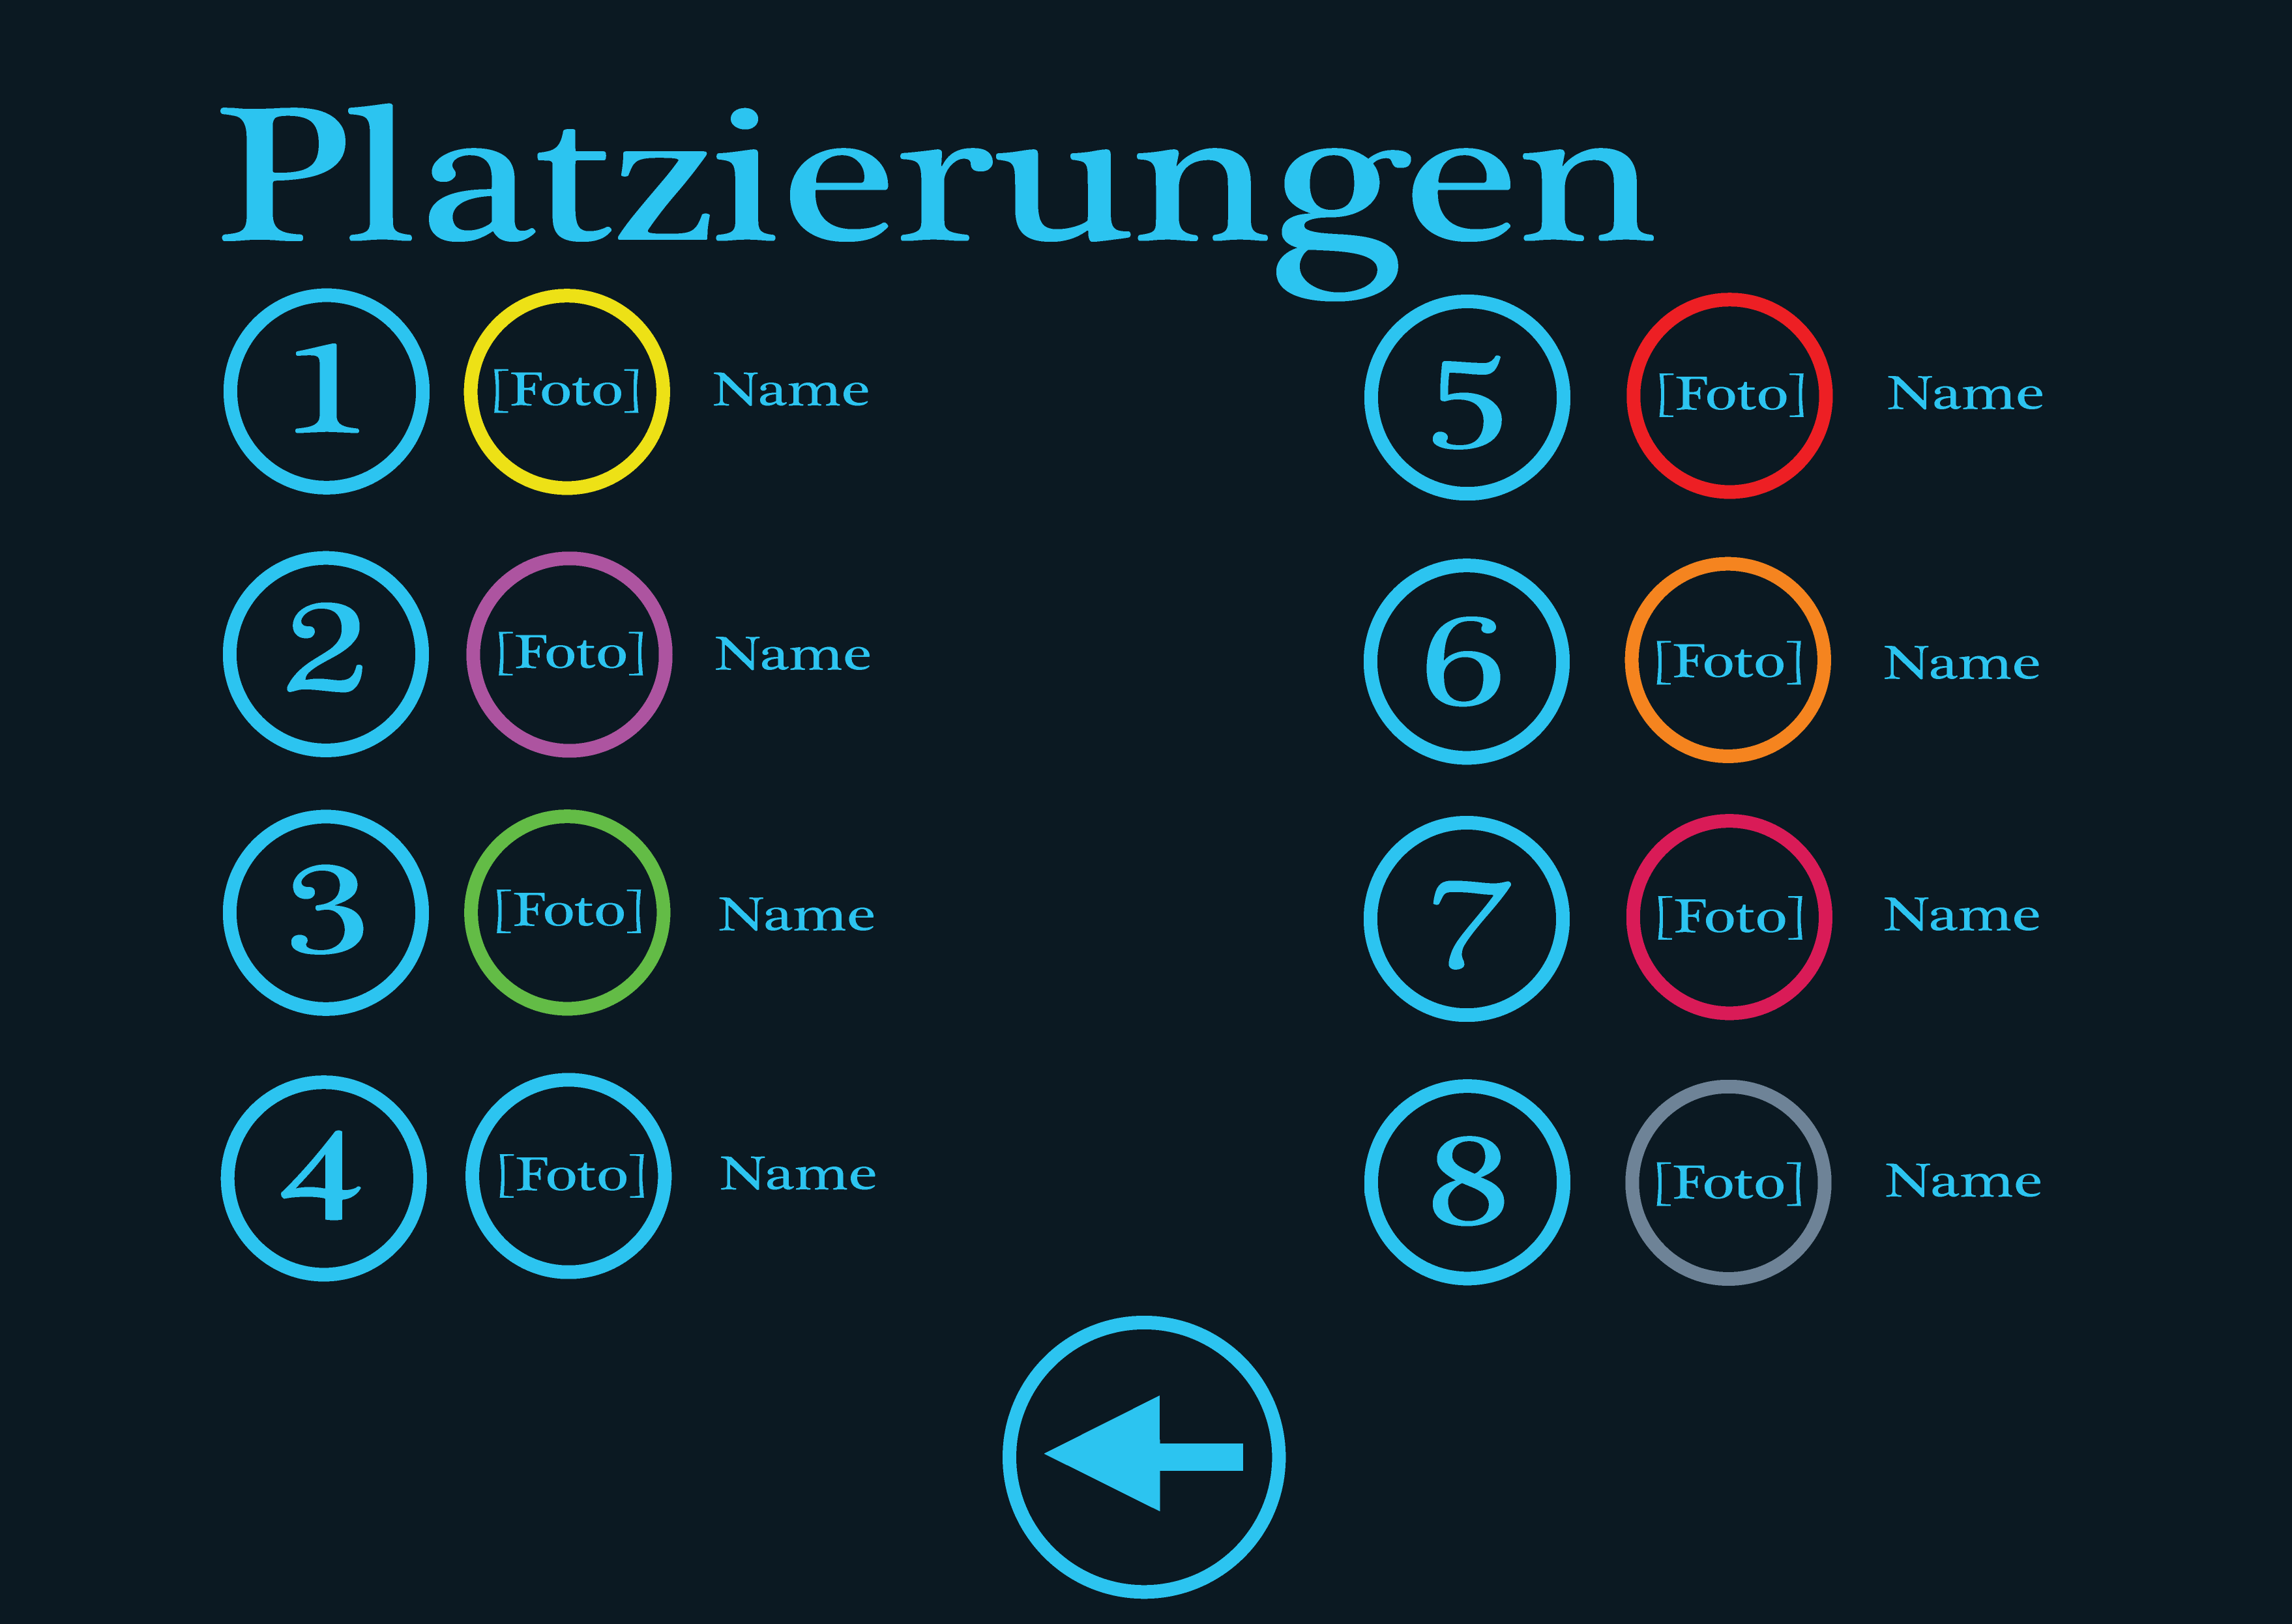
\includegraphics[width=0.9\textwidth]{img/platzierungen.png}\\
\textit{Platzierungen nach Ende des Rennens}

\newpage

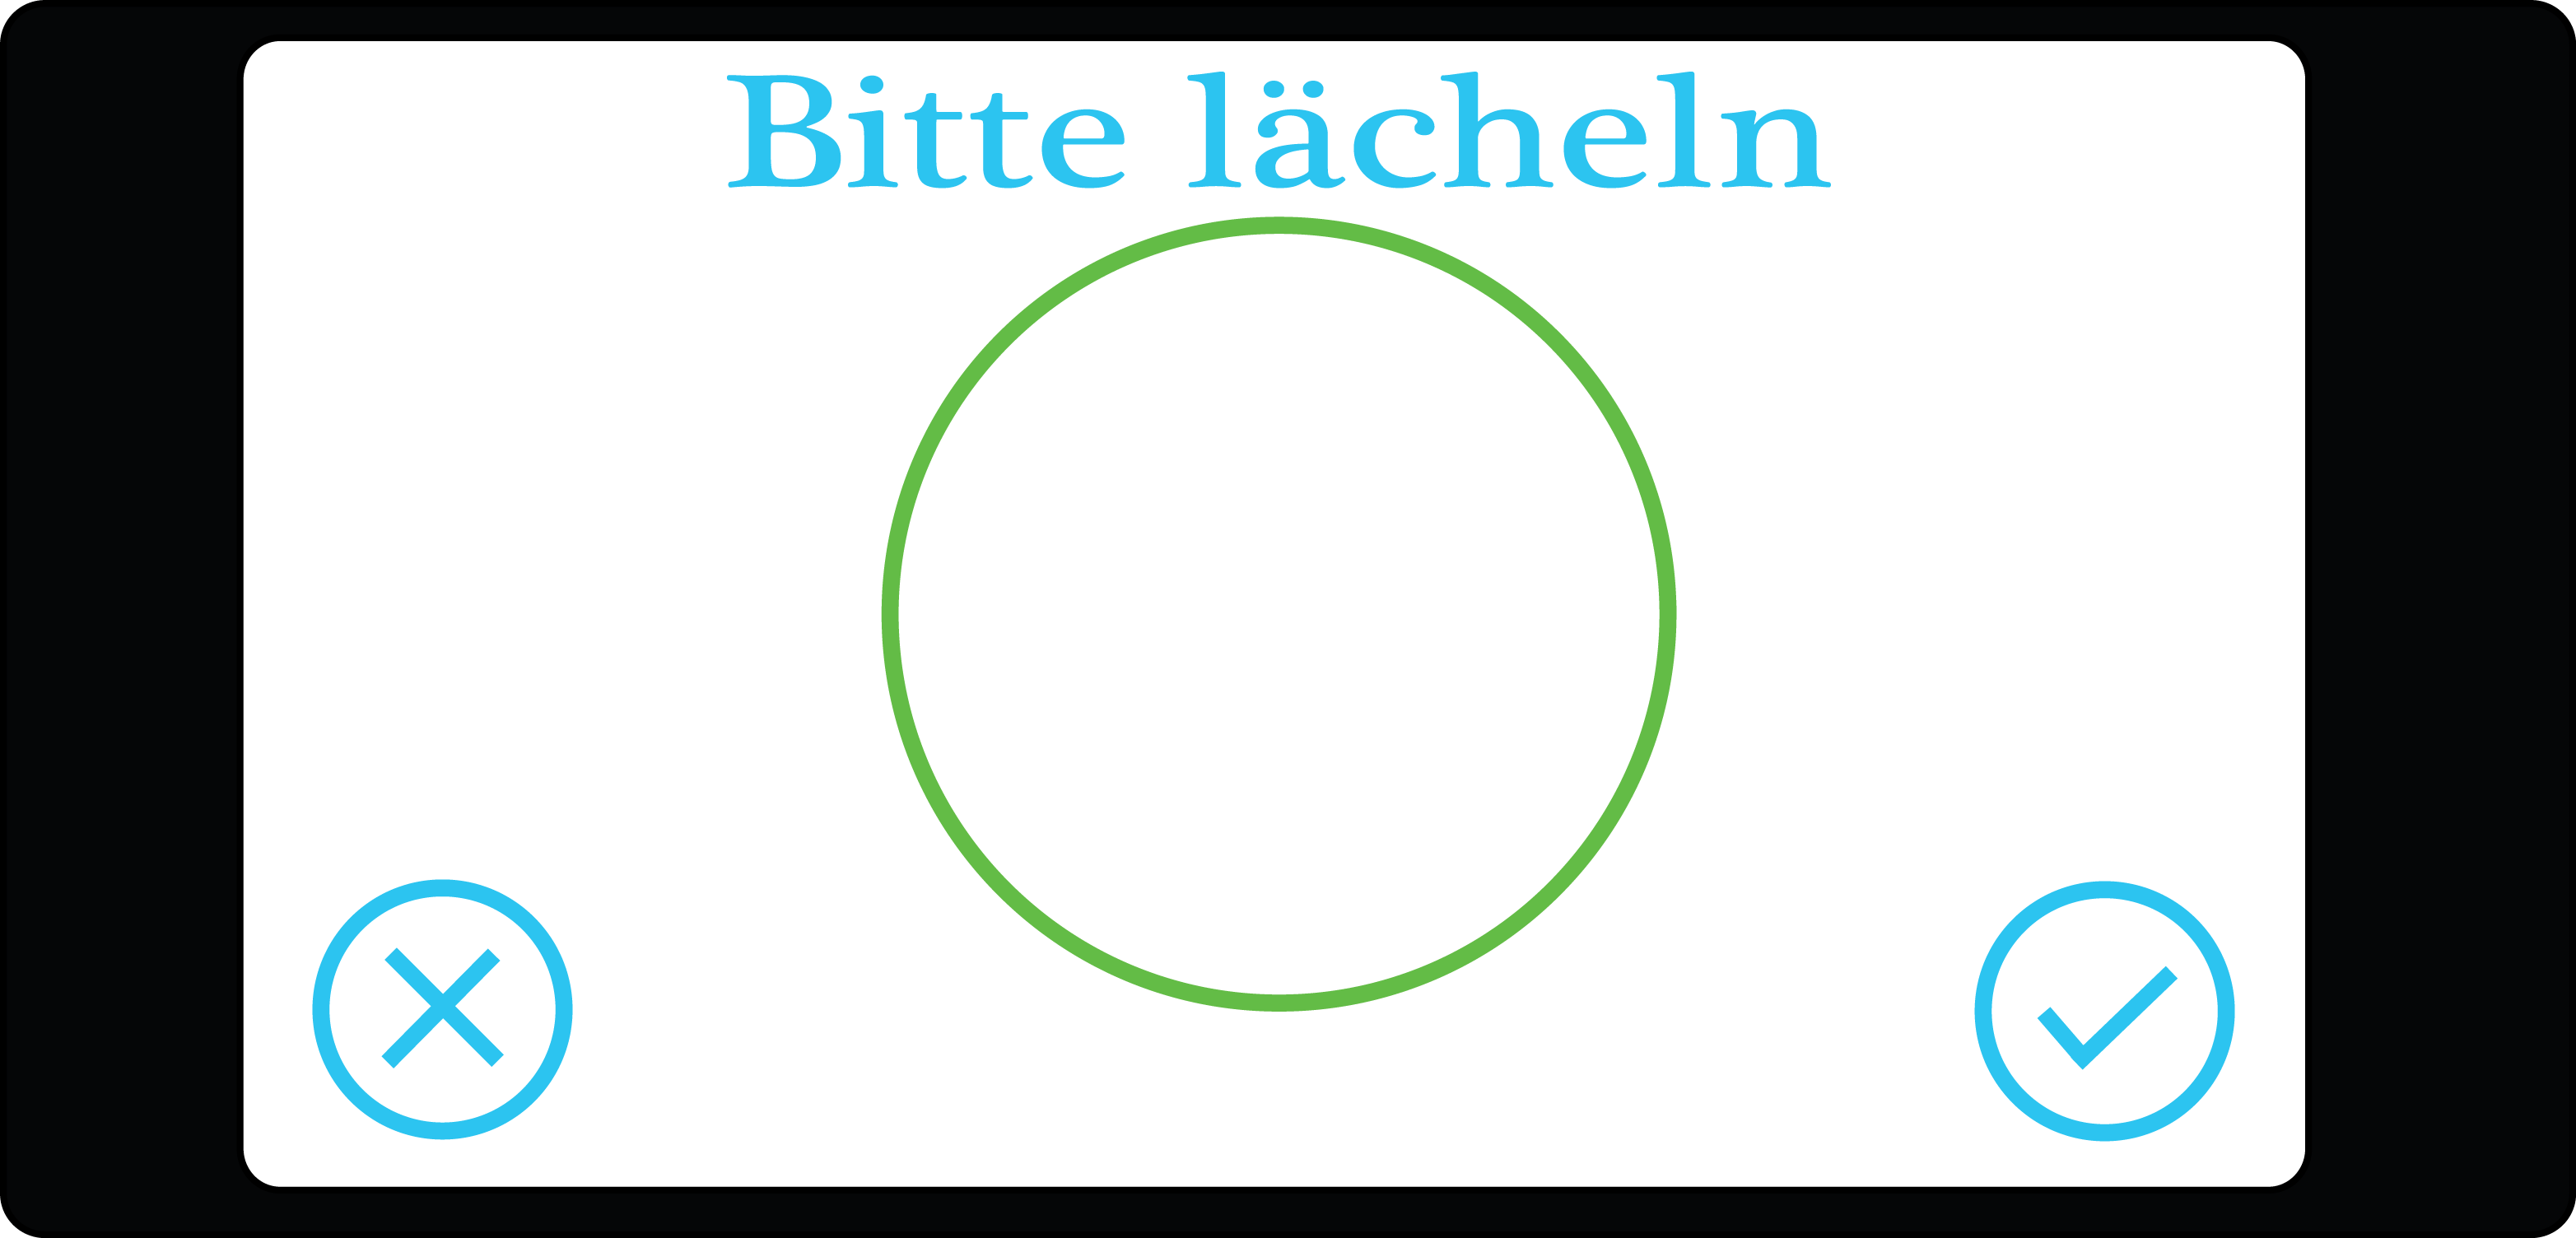
\includegraphics[width=0.9\textwidth]{img/profilbild_erstellen.png}\\
\textit{Profilbild erstellen}\\[4em]

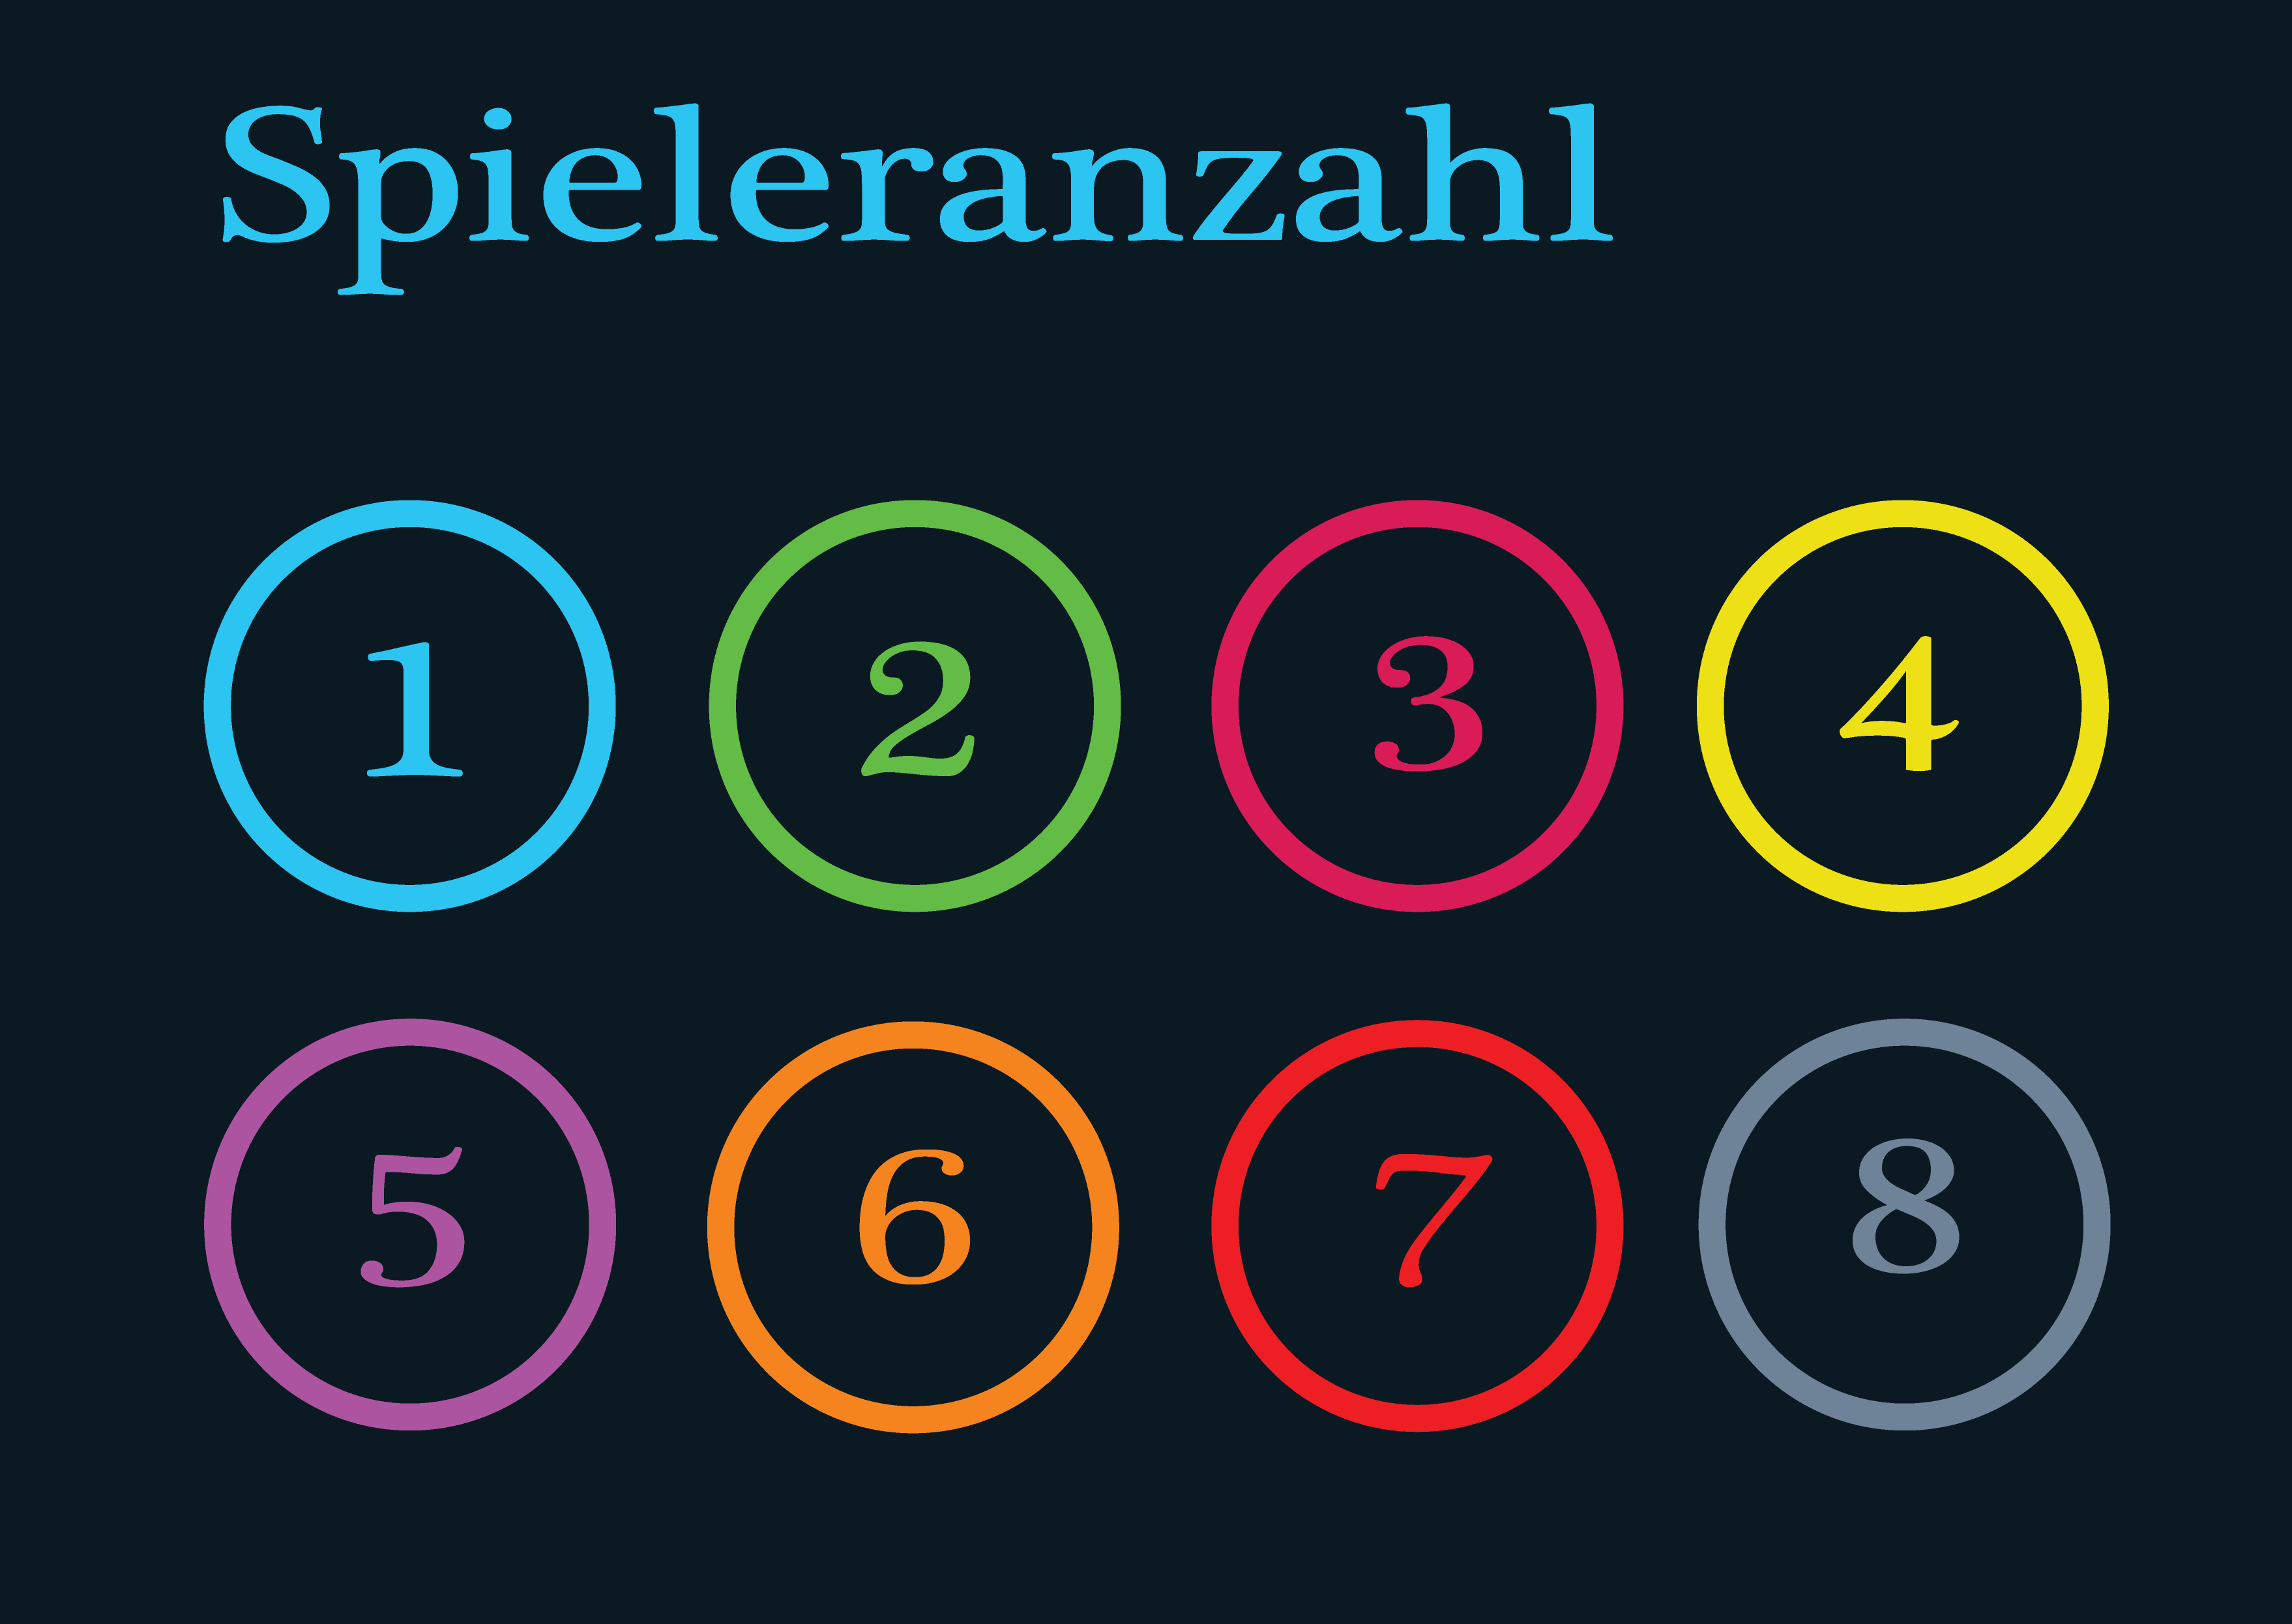
\includegraphics[width=0.9\textwidth]{img/spieleranzahl.png}\\
\textit{Anzeige der Spieleranzahl}

\newpage

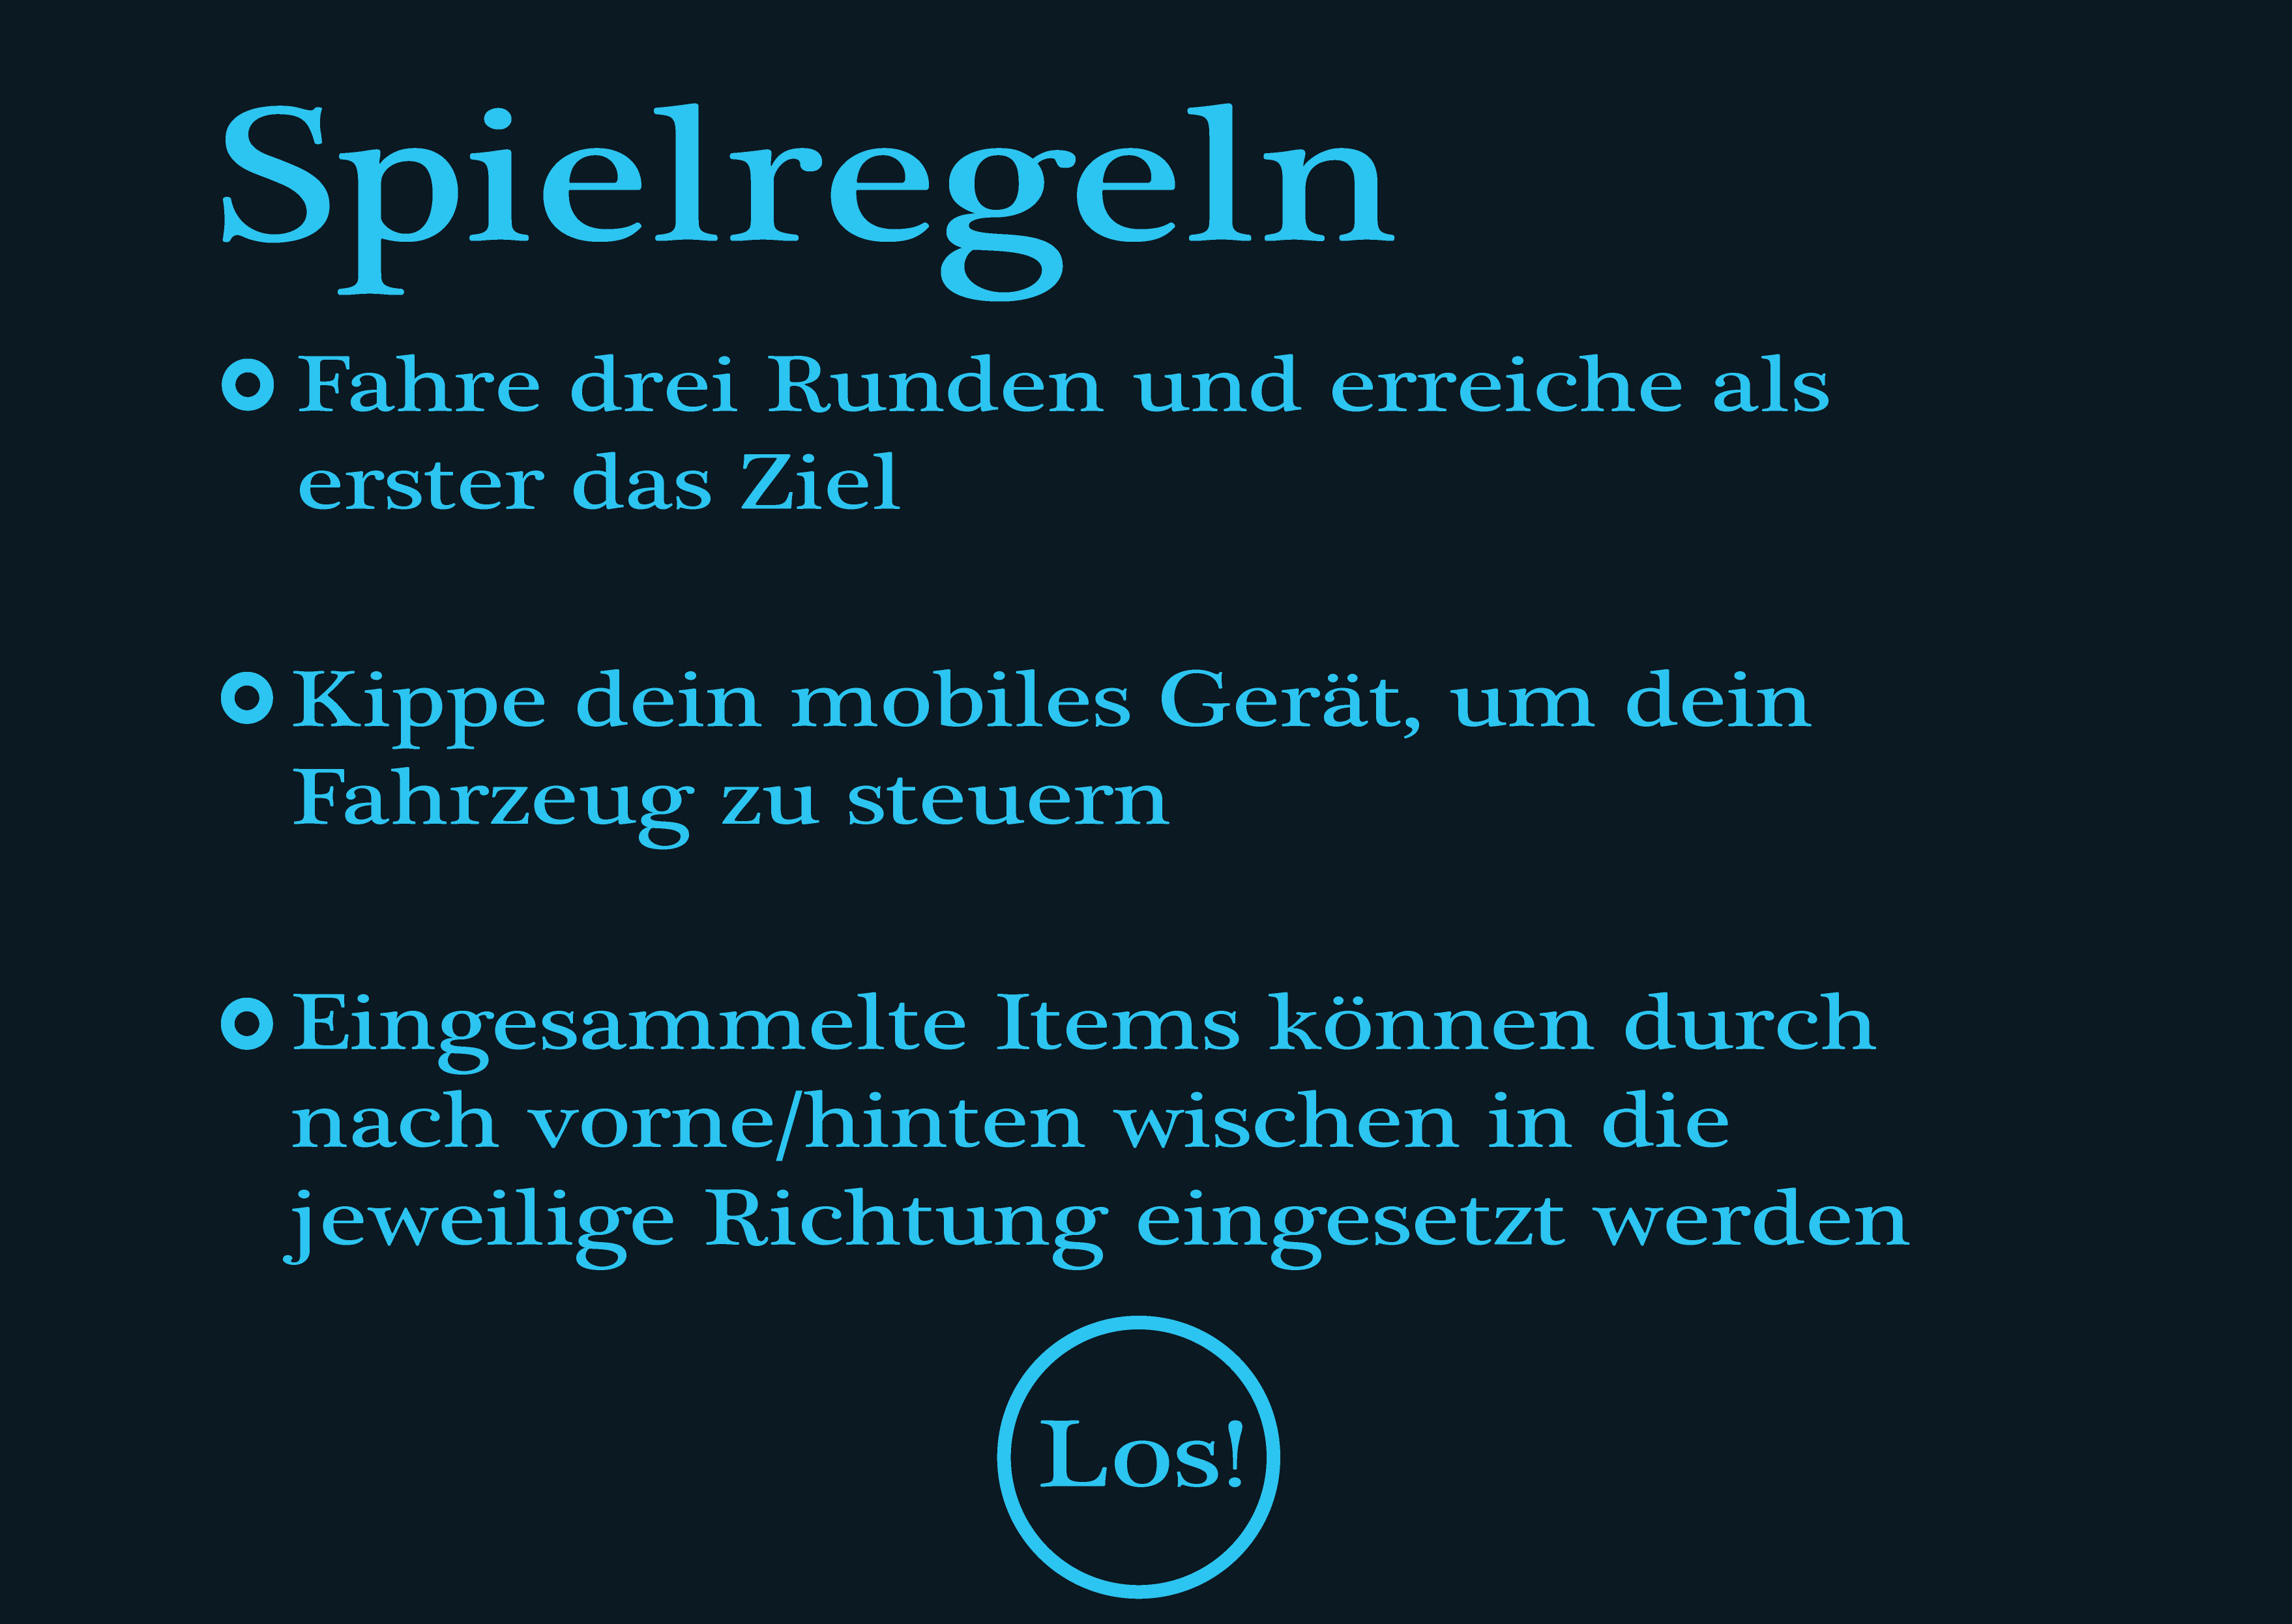
\includegraphics[width=0.9\textwidth]{img/spielregeln.png}\\
\textit{Die Spielregeln}\\[2em]


\includegraphics[width=0.9\textwidth]{img/win.png}\\
\textit{Die Anzeige des Siegers}

\end{flushright}
